\section{Infinite Lattice Multiplication Factor}
\label{sec:infinite_lattice}

\subsection{Problem Statement}
\label{subsec:infinite_lattice_ps}

In an infinite lattice a reactor of infinite size is considered and therefore neutrons are not capable of leaking out of the system. An infinite lattice effectively removes the effects of geometry in neutron transport and characterizes the system entirely in terms of its material properties. Since the physics of an infinite lattice are greatly simplified an analytic analysis of the system is possible. Consequently, the infinite lattice problem is ideal for an initial analysis of any new computational method. 

To begin, the mathematical formulation of an infinite lattice will be described. In matrix form the two-group neutron balance equations for an infinite lattice can be written as,
\begin{equation}
\label{eq:infinite_lattice_neutron_balance}
   \left(
    \begin{array}{cc}
     \Sigma_{a_1} + \Sigma_{1\rightarrow 2} & 0 \\
     -\Sigma_{12} & \Sigma_{a_2} 
    \end{array}
   \right)
   \left(
    \begin{array}{c}
     \phi_1 \\
     \phi_2
    \end{array}
   \right) 
   = \frac{1}{k_{\infty}}
   \left(
    \begin{array}{cc}
     \nu\Sigma_{f_1} & \nu\Sigma_{f_2} \\
     0 & 0 
    \end{array}
   \right)
   \left(
    \begin{array}{c}
     \phi_1 \\
     \phi_2
    \end{array}
   \right). 
\end{equation}  
Solving the system in \ref{eq:infinite_lattice_neutron_balance} for the infinite multiplication factor, the following analytic expression is obtained,
\begin{equation}
\label{eq:infinite_lattice_kinf}
   k = \frac{\Sigma_{a_2}\nu\Sigma_{f_1} + 
             \Sigma_{1\rightarrow 2}\nu\Sigma_{f_2}}{
              \Sigma_{a_2}\left(
               \Sigma_{a_1} + \Sigma_{1\rightarrow 2}\right)}.
\end{equation}
The infinite multiplication factor is a function of five material parameters. Since this thesis is concerned with the affect of uncertainties in input parameters on computer code outputs, variations in $k_{\infty}$ as a function its stochastic input variables are of interest. Assume all variation in $k_{\infty}$ can be attributed to its input cross sections, whose distributions follow a multivariate Gaussian. To obtain physical homogenized, two-group cross section values a real system must first be modeled in a transport code. The \ac{UAM} Benchmark is sought for this purpose \cite{UAM_Benchmark}. Specifically, the \ac{TMI} assembly is modeled using the two-step method described in \cite{TwoStep_Approach}. A total of 300 perturbed cross section sets were produced to obtain the few-group mean and covariance data used in the proceeding analysis. The cross section data is summarized in Table \ref{table:infintie_lattice_tmi_data}.      
\begin{table}[!htb]
\caption[TMI infinite lattice two-group cross sections.]{\label{table:infintie_lattice_tmi_data} 
Two-group cross section data for an infinite TMI lattice.}
\centering
\begin{tabular}{||c||c|c|c|c|c|c|c||} 
\hline \hline
  &  &  & \multicolumn{5}{|c||}{\textbf{Correlation Coefficient Matrix}}  \\ \hline
  & \textbf{Mean} & \textbf{Standard Dev.} & $\Sigma_{a_1}$ & $\Sigma_{a_2}$ & 
  $\nu\Sigma_{f_1}$ & $\nu\Sigma_{f_2}$ & $\Sigma_{1\rightarrow 2}$ \\ \hline \hline
$\Sigma_{a_1}$ & 1.04E-02 & 9.06E-05 & 1 & 0.07 & -0.13 & 0.02 & 0.75 \\ \hline
$\Sigma_{a_2}$ & 1.10E-01 & 2.31E-04 & 0.07  &  1     & 0.06  & 0.31 & -0.07 \\ \hline
$\nu\Sigma_{f_1}$ & 9.00E-03 & 4.85E-05 & -0.13 &  0.06  & 1     & 0.33 & -0.10 \\ \hline
$\nu\Sigma_{f_2}$ & 1.91E-01 & 8.87E-04 & 0.02  &  0.31  & 0.33  & 1    & 0.01 \\ \hline
$\Sigma_{1\rightarrow 2}$ & 1.80E-02 & 2.18E-04 & 0.75  &  -0.07 & -0.10 & 0.01 & 1 \\ \hline \hline
\end{tabular}
\end{table}

Multiple methods will be applied to obtain basic statistical and sensitivity data on the infinite multiplication factor. Of course, Monte Carlo sampling using the input cross sections' covariance matrix and applying \ref{eq:sample_covariance} will provide the mean and variance of $k_{\infty}$. Another approach to get at the variance of $k_{\infty}$ is through the "Sandwich Equation"\cite{Jessee_Turinsky},
\begin{equation}
\label{eq:sandwich}
   \sigma^2(k_{\infty}) = S^TCS
\end{equation}      
where $C$ is the covariance matrix for the input data. In equation \ref{eq:sandwich} the array $S$ contains sensitivities of the output to the input parameters. For this problem the vector $S$ contains,
\begin{equation}
\label{eq:sensitivity_vector}
   S^T = \left(
    \begin{array}{ccccc}
     \frac{\partial k_{\infty}}{\partial\Sigma_{a_1}} &
     \frac{\partial k_{\infty}}{\partial\Sigma_{a_2}} &
     \frac{\partial k_{\infty}}{\partial\nu\Sigma_{f_1}} &
     \frac{\partial k_{\infty}}{\partial\nu\Sigma_{f_2}} &
     \frac{\partial k_{\infty}}{\partial\Sigma_{1\rightarrow 2}}
    \end{array}
         \right).
\end{equation} 
Since there exists an analytic expression for $k_{\infty}$ the sensitivity vector for this problem in \ref{eq:sensitivity_vector} is exact. As a side-check the sensitivity vector $S$ can also be constructed using central differencing. The sensitivity of $k_{\infty}$ to the $i^{\text{th}}$ cross section $\Sigma_i$ using central differencing is expressed as, 
\begin{equation}
\label{eq:central_diff_kinf}
   \frac{\partial k_{\infty}}{\partial \Sigma_i}\biggr\rvert_
   {\Sigma_{j\neq i} = \bar{\Sigma}_j}
    \approx \frac{k_{\infty}(\Sigma_i + \Delta\Sigma_i) - 
    k_{\infty}(\Sigma_i - \Delta\Sigma_i)}
    {2\Delta\Sigma_i}
\end{equation} 
where all cross sections $\Sigma_j$, $j\neq i$, are held at their mean values. Generally a one percent perturbation $\Delta\Sigma$ is sufficient to obtain accurate sensitivities although this rule of thumb is dependent on the smoothness of the objective function. With a variety of methods available to obtain sensitivities and statistical moments of $k_{\infty}$ it is possible to thoroughly assess the potential of a reduced order model.       
     
\subsection{Analysis}
\label{subsec:kinf_analysis}

Several elements of the methodologies described in Chapter \ref{chap:rom} will be tested in this section and compared to results obtained using analytic and Monte Carlo approaches. For all Smolyak sparse grids constructed the hypercube domain extends to six standard deviations in each random variable. Since $k_{\infty}$ is a function of only five random variables a sparse grid interpolant will be constructed without applying any function decomposition in order to demonstrate the accuracy and convergence of the method. The convergence criteria for the sparse grid interpolant is set such that the maximum hierarchical surplus at a given level is not to exceed $10^{-10}$. Both Clenshaw-Curtis and Gauss-Patterson abscissas are tested. 
\begin{figure}
\caption[Hierarchical surplus convergence for infinite TMI lattice.]{ \label{fig:kinf_sg_convergence}
Convergence study of a five dimensional sparse grid interpolant for the  multiplication factor of an infinite TMI lattice. The boxed numbers represent the current number of knots in the sparse grid.}
 \begin{center}
  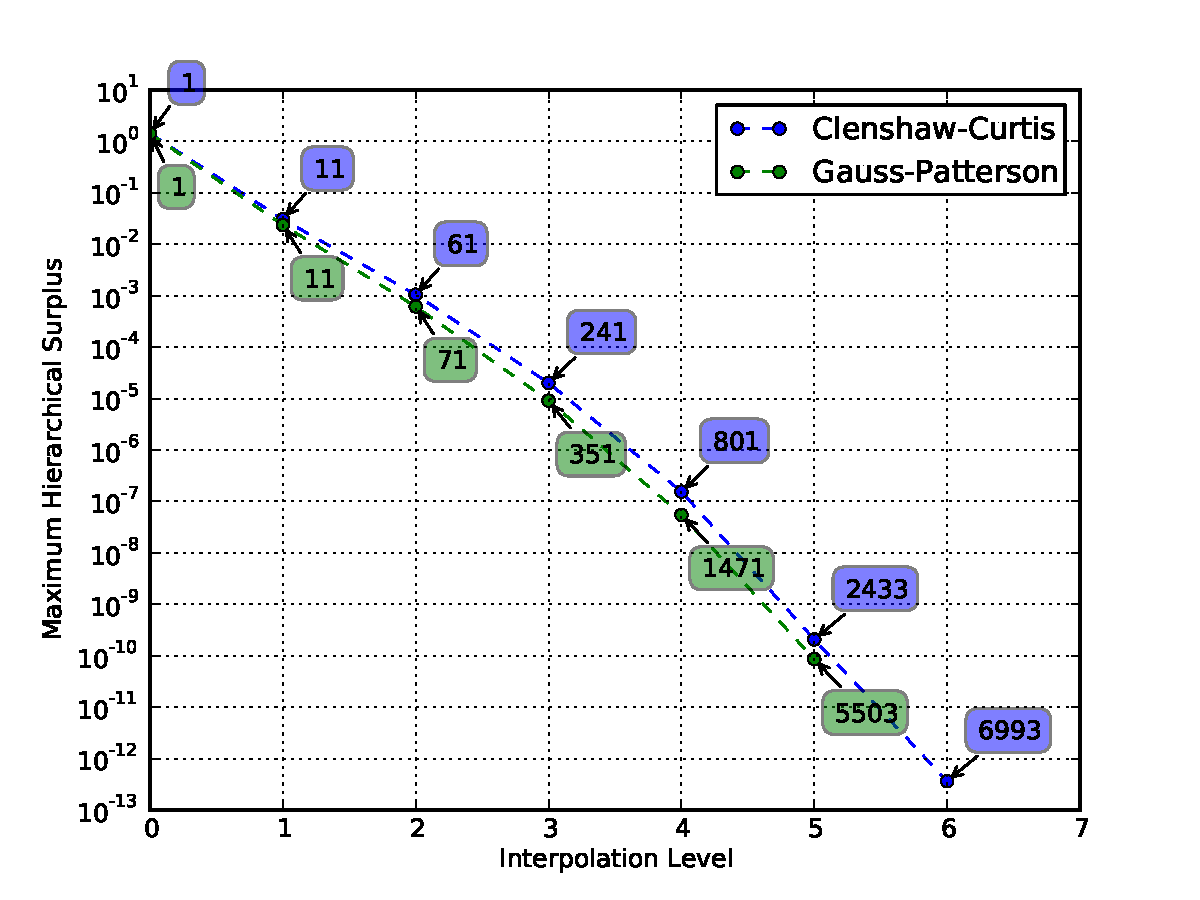
\includegraphics[scale=.75]{./Chapter3/kinf_sparse_grid_convergence.pdf}
 \end{center}
\end{figure}

From Fig. \ref{fig:kinf_sg_convergence} the Clenshaw-Curtis and Gauss-Patterson schemes perform similarly in terms of level to level convergence. However, observe that at each interpolation level the Gauss-Patterson scheme requires significantly more nodes in exchange for a small increase in convergence speed. Both schemes converge to the threshold around level five although the Gauss-Patterson scheme requires more than twice as many function evaluations to get there than Clenshaw-Curtis. Based on the graphical determination of order of convergence \cite{Boyd}, it is clear from \ref{fig:kinf_sg_convergence} that the Smolyak interpolant for $k_{\infty}$ converges geometrically.

With the Smolyak interpolation routines working as expected it's safe to apply them to an anchored-\ac{ANOVA} decomposition of $k_{\infty}$. To start, only the first order components will be built and analyzed. The first order components are relatively cheap to produce and often collectively produce very accurate reduced order models \cite{AHSGC_HighDimensions}. Afterwards, all higher order components will be added in order to show that the full anchored-\ac{ANOVA} decomposition can fully reproduce the objective function. Since $k_{\infty}$ is a function of only five random variables there is no point in adaptively constructing the reduced order model as described in Section \ref{subsec:dimension_truncation}.        

As a first comparison between all the models developed for quantifying the uncertainty in $k_{\infty}$ the mean and variance values of each model will be compared. With the exception of the variance obtained using the Sandwich Equation, each model's variance was obtained by propagating 1000 samples of Eq. $\ref{eq:sample_covariance}$ through the model. All samples produced for each model were seeded identically and so the same random numbers were drawn. The mean and variance results, along with 99\% confidence intervals, are summarized in Table \ref{table:kinf_mean_variance}. 
    
\begin{table} 
\caption[Mean and variance for TMI infinite multiplication factor.]{\label{table:kinf_mean_variance} 
Mean and variance data for the multiplication factor of an infinite TMI lattice obtained using Monte Carlo sampling. Wherever sampling was utilized the same random numbers were used.}
\centering
\small
\begin{tabular}{||c|c|c|c|c||} 
\hline \hline
\textbf{Method} & \textbf{Mean} & \textbf{99\% CI} & \textbf{Standard Dev.} & \textbf{99\% CI} \\ \hline
5D Sparse Grid CC      & 1.41562 & (1.41512, 1.41612) & 0.006168 & (0.005909, 0.006544) \\ \hline
5D Sparse Grid GP      & 1.41562 & (1.41512, 1.41612) & 0.006168 & (0.005831, 0.006544) \\ \hline
1D ANOVA CC  & 1.41560 & (1.41510, 1.41610) & 0.006168 & (0.005831, 0.006544) \\ \hline
All ANOVA CC & 1.41562 & (1.41512, 1.41612) & 0.006168 & (0.005831, 0.006544) \\ \hline
1D ANOVA GP  & 1.41560 & (1.41510, 1.41610) & 0.006168 & (0.005831, 0.006544) \\ \hline
All ANOVA GP & 1.41562 & (1.41512, 1.41612) & 0.006168 & (0.005831, 0.006544) \\ \hline
True Function & 1.41562 & (1.41512, 1.41612) & 0.006168 & (0.005831, 0.006544) \\ \hline
Sandwich               &         &                    & 0.006540 &                      \\
\hline \hline
\end{tabular}
\end{table}

The five dimensional sparse grid interpolant results are entirely self consistent with the anchored-\ac{ANOVA} results. Further, both of these methods produce identical results to those obtained using Monte Carlo sampling. Although the analytic variance from the Sandwich Equation is within the 99\% confidence bounds of each model's results, there is a notable difference due to the fact that only 1000 samples were used to obtain each model's statistics. Increasing the number of samples decreased the difference. Note that in Table \ref{table:kinf_mean_variance} the anchored-\ac{ANOVA} the reduced order models consisting of only one dimension anchored-\ac{ANOVA} components perform just as well as the full decomposition and the sparse grid interpolants over all five random variables. However, the 1D component models require only 29 function evaluations to produce, which is some ten times fewer evaluations than the 5D interpolants, and some hundred times fewer evaluations than the full decomposition. 
\begin{figure}
\caption[Cumulative knot count for constructing an anchored-\ac{ANOVA} decomposition.]{ \label{fig:kinf_numknots}
Cumulative number of knots required at each level of an anchored-\ac{ANOVA} decomposition of the multiplication factor of an infinite TMI lattice. Boxes contain the calculated standard deviation at the current level.}
 \begin{center}
  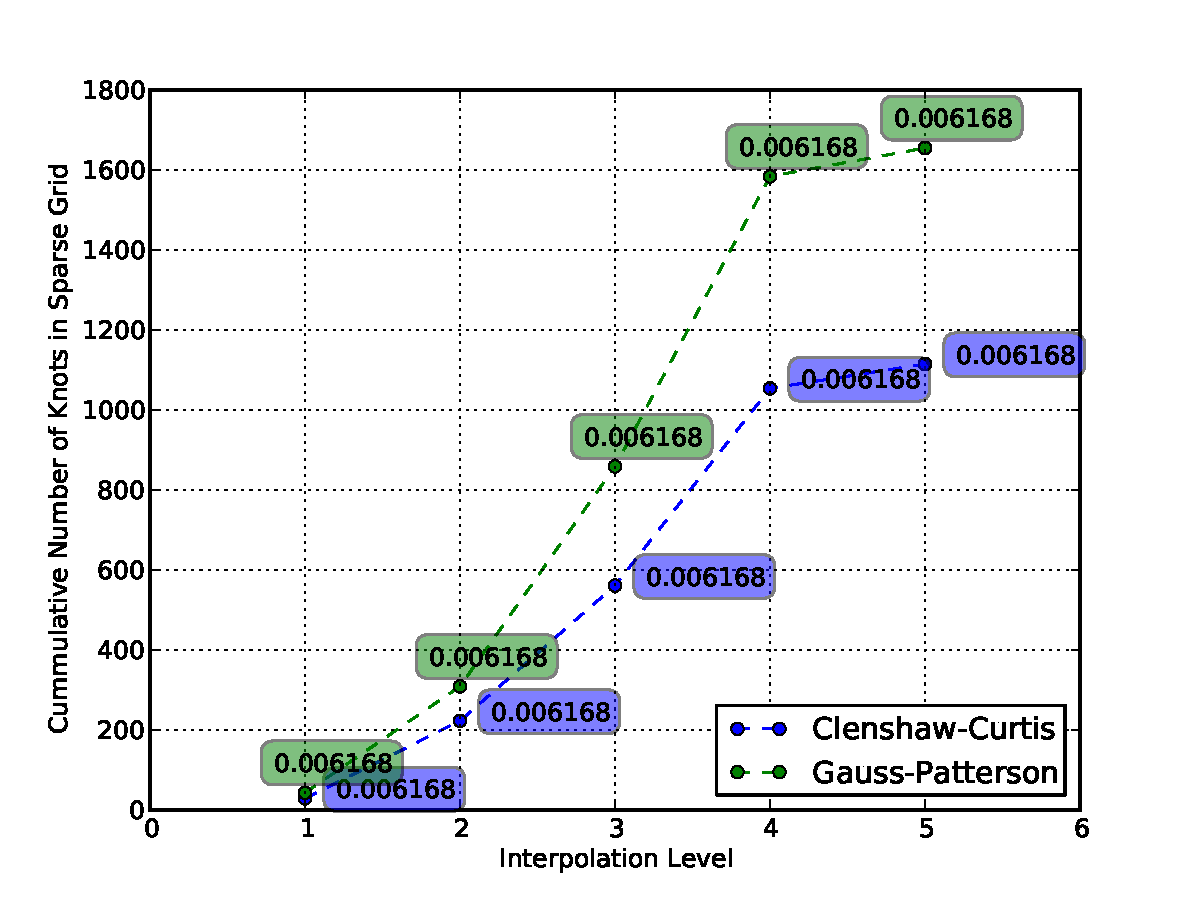
\includegraphics[scale=.75]{./Chapter3/kinf_sparse_grid_numknots.pdf}
 \end{center}
\end{figure}
The rapid convergence of the reduced order model containing only one dimensional anchored-\ac{ANOVA} components is shown in \ref{fig:kinf_numknots}. Construction of higher order components is very expensive. Fortunately for this problem, and perhaps others, construction of only one dimensional components is completely sufficient to represent the objective function. 

As another performance measure of the reduced order model methodologies, each model is used to obtain normalized sensitivity coefficients for $k_{\infty}$. Central differencing is applied to each model, with perturbations made to each cross section at a time while holding the other cross sections at their mean values. Perturbations are taken to be 1\% of each cross section's value. Using the analytic expression for $k_{\infty}$ in \ref{eq:infinite_lattice_kinf}, the central differencing results can be compared to the true sensitivity coefficients.   The results are summarized in Table \ref{table:kinf_sensitivities}. Table \ref{table:kinf_sensitivities}, sensitivity coefficients are also obtained by applying central differencing to the true function as in Eq. \ref{eq:central_diff_kinf}. 
\begin{table}
\caption{\label{table:kinf_sensitivities} 
Normalized sensitivity coefficients for the multiplication factor of an infinite TMI lattice.}
\centering
\begin{tabular}{||c|c|c|c|c|c||} 
\hline \hline
  & \multicolumn{5}{|c||}{\textbf{Normalized Sensitivity Coefficient of $k_{\infty}$}}  \\ \hline
\textbf{Method} & $\Sigma_{a_1}$ & $\Sigma_{a_2}$ & $\nu\Sigma_{f_1}$ & $\nu\Sigma_{f_2}$ & $\Sigma_{1\rightarrow 2}$ \\ \hline
5D Sparse Grid CC  & -.367551 & -.776087 & .224060 & .776010 & .143491 \\ \hline
5D Sparse Grid GP  & -.367551 & -.776087 & .224060 & .776010 & .143491 \\ \hline
1D ANOVA CC        & -.367556 & -.776098 & .224063 & .776020 & .143493 \\ \hline
All ANOVA CC       & -.367551 & -.776087 & .224060 & .776010 & .143491 \\ \hline
1D ANOVA GP        & -.367556 & -.776098 & .224063 & .776020 & .143493 \\ \hline
All ANOVA GP       & -.367551 & -.776087 & .224060 & .776010 & .143491 \\ \hline
Analytic           & -.367520 & -.775956 & .224044 & .775956 & .143476 \\ \hline
Central Difference & -.367551 & -.776089 & .224060 & .776011 & .143492 \\
\hline \hline
\end{tabular}
\end{table}
As expected, all models utilizing the central differencing formula produce self consistent sensitivity coefficients. The models differ from the analytic sensitivity coefficients only in the fourth decimal place, which is expected given the $\mathcal{O}(\Delta\Sigma^2)$ convergence  of the central differencing formula.     